\subsection{R 的连通子集}

定理 4. R 的子集 A 连通当且仅当 A 是区间。 1) 条件是必要的。设 A 连通：若 A 由单独一点组成，它是一个区间。若 A 多于

一点，设 \(a\) 与 \(b\) 是 A 中满足 \(a < b\) 的两点；由第 4 目的命题 1，只需证明每个这样的 \(x\) （ \(a < x < b\) ）都属于 A。现在，若 \(x \notin A\) ，我们将有 \(A \subset \mathbb{C}\{x\}\) ；但 \(\mathbb{C}\{x\}\) 是两个不相交开集 \([] \leftarrow, x[\) 与 \(]x, \rightarrow[\) 的并，其中每个都与 A 相交，因而 A 将不连通，与假设矛盾。 2) 条件是充分的。先证每个紧区间 \([a, b]\) 连通。对每个整数 \(n > 0\) ，令 \(V_{1/n}\) 为由所有对 \((x, y)\) （满足 \(|x - y| \leqslant 1/n\) ）组成的一致邻域；由第二章 § 4 第 4 目的命题 6，只需证明每一对点 \(x, y\) （ \([a, b]\) 的）都能用一条 \(V_{1/n}\) -链连接。设 \(p\) 是使 \(p/n \leqslant x\) 的最大整数，\(q\) 是使 \(q/n \leqslant y\) 的最大整数（由第 1 目的定理 1，\(p\) 与 \(q\) 存在）；则 \(p \leqslant q\) 。若 \(p = q\) ，则 \(y - x < 1/n\) ，点 \(x\) 与 \(y\) 组成一条 \(V_{1/n}\) -链。若 \(q > p\) ，令 \(x_i = (p + i)/n\) （ \(i = 1, 2, \ldots, q - p\) ）；我们有 \(x_1 - x \leqslant 1/n\) ，\(y - x_{q-p} \leqslant 1/n\) 且 \(x_{i+1} - x_i = 1/n\) ，于是点 \(x, x_1, x_2, \ldots, x_{q-p}, y\) 组成一条 \(V_{1/n}\) -链，连接 \(x\) 与 \(y\) 。

现在若 I 是不由单独一点组成的任一区间，且 \(a\) 与 \(b\) 是 I 中满足 \(a < b\) 的任意两点，则区间 \([a, b]\) 含于 I 且连通，因而 I 连通。

推论 1. 实直线是连通且局部连通的空间。

推论 2. R 的紧连通子集只有有界闭区间。

由定理 4，不含任何由多于一点组成的区间的 R 的子集是全不连通的；例如有理数集 Q 就是如此，因为无理数集 \(\mathbb{Q}\) 在 R 中稠密。

命题 2. R 中每个非空开集是可数个两两不相交的开区间所成的族之并。

设 A 是 R 中的非空开集。由于 R 局部连通，A 的每个分支都是连通开集（第一章 § 11 第 6 目，命题 11），因而由定理 4 是开区间。这些开区间中任何两个都不相交；另一方面，每个都含有理数；因此这些区间组成的集的势小于或等于 Q 的势，即是可数的。

由此推出 R 中每个闭集是两两不相交的开区间（有限或无限）序列 \((I_{n})\) 的并的余集。这些区间称为与所考虑的闭集邻接。反之，给定这样一个区间序列，它们的并的余集是一个闭集，而这些区间与它邻接。

例. 我们用归纳法定义可数个两两不相交的开区间所成的族 \((I_{n,p})\) 如下：

整数 \(n\) 取遍所有 \(\geqslant 0\) 的值，而对每个值 \(n, p\) 取值 \(1, 2, 3, \ldots, 2^n\) 。所有区间 \(I_{n,p}\) 都含于

\[
\mathbf {A} = [ \mathbf {0}, \mathbf {1} ],
\]

而我们取 \(\mathbf{I}_{0,1} = ]1/3, 2/3[\) （ {]}0, 1{[} 的“中间三分之一”）。现在设 \(2^{m+1} - 1\) 个区间 \(\mathbf{I}_{n,p}\) （对 \(0 \leqslant n \leqslant m\) ）已经定义，使得：若 \(\mathbf{J}_m\) 是它们的并，则集 \(\mathbf{A} \cap \complement_{\mathbf{J}_m}\) 是 \(2^{m+1}\) 个两两不相交的闭区间 \(\mathbf{K}_{m,p}\) （ \(1 \leqslant p \leqslant 2^{m+1}\) ）的并，每个长为 \(\frac{1}{3^{m+1}}\) 。若 \(\mathbf{K}_{m,p} = [a, b]\) ，则取 \(\mathbf{I}_{m+1,p}\) 为开区间 \(\left]a + \frac{b - a}{3}, b - \frac{b - a}{3}\right[\) （区间 {]}a, b{[} 的“中间三分之一”），并且立即可以验证归纳能如此继续下去（图 3）。

\pandocbounded{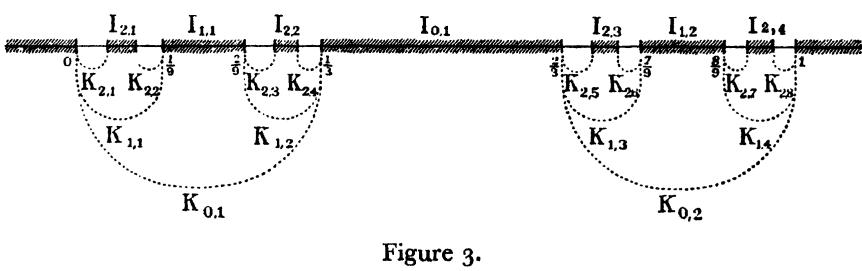
\includegraphics[keepaspectratio]{images/part002_c6c4994f.jpg}}\\
图 3。
若 \(\mathbf{K}'\) 是诸 \(\mathbf{I}_{n,p}\) 的并的余集，则闭集 \(\mathbf{K} = \mathbf{A} \cap \mathbf{K}'\) 称为 Cantor 三分集。显然 \(\mathbf{K}\) 是紧的（第 2 目，定理 2）；而且 \(\mathbf{K}\) 是全不连通的。因为若 \(\mathbf{K}\) 包含一个长度 \(>0\) 的区间 I，则 I 将含于某个区间 \(\mathbf{K}_{m,p}\) ；于是它的长度将 \(\leqslant 1/3^{m+1}\) 对每个 \(m\) 成立，这是荒谬的。

